\documentclass[aspectratio=169, 11pt]{beamer}

% --- Tema y colores ---
\usetheme{Madrid}
\usecolortheme{seahorse}
\setbeamertemplate{navigation symbols}{}
\setbeamertemplate{footline}[frame number]

% --- Codificación y lenguaje ---
\usepackage[utf8]{inputenc}
\usepackage[T1]{fontenc}
\usepackage[spanish]{babel}

% --- Paquetes ---
\usepackage{amsmath, amssymb}
\usepackage{graphicx}
\usepackage{booktabs}
\usepackage{xcolor}
\usepackage{colortbl}
\usepackage{tikz}
\usetikzlibrary{arrows.meta, positioning, shapes.geometric, calc}

% --- Metadata ---
\title[STFT vs CWT en EEG-Alzheimer]{%
    ¿Importa cómo descomponemos el EEG para detectar Alzheimer?}
\subtitle{Replicación de Lopes et al.~2023 y comparación STFT vs CWT-Morlet}
\author{Sebastián Palacio Betancur}
\institute[UNAL]{%
    Universidad Nacional de Colombia --- Sede Medellín \\
    Facultad de Minas \\[4pt]
    \textit{Tópicos en Procesamiento Digital de Señales} \\
    Prof.\ Freddy Bolaños}
\date{Junio de 2026}

\begin{document}

% ============================================================
% SLIDE 1: Título
% ============================================================
\begin{frame}
\titlepage
\end{frame}

% ============================================================
% SLIDE 2: La pregunta (hook)
% ============================================================
\begin{frame}{La pregunta}

\begin{columns}[T]
\begin{column}{0.56\textwidth}
\begin{itemize}
    \item El Alzheimer es la demencia \#1 ($>$55 M personas). Detectarlo
    temprano es clave, pero MRI/PET son caros.
    \item El \textbf{EEG} es barato y portátil. Su
    \textbf{espectrograma de modulación} captura \emph{a qué ritmo}
    cambia la energía en cada banda --- un biomarcador prometedor.
    \item Todo depende del primer paso: la \textbf{descomposición
    tiempo-frecuencia}.
\end{itemize}

\vfill
\begin{block}{Hipótesis}
\small La \textbf{CWT}, con mejor resolución en bajas frecuencias,
debería superar a la \textbf{STFT} para el Alzheimer.
\end{block}
\end{column}
\begin{column}{0.40\textwidth}
\centering
\begin{tikzpicture}[
    box/.style={draw, rounded corners, fill=blue!10, minimum width=2.8cm,
                minimum height=0.75cm, align=center, font=\small},
    arr/.style={-{Stealth[length=2.5mm]}, thick}
]
\node[box] (eeg) {Señal EEG\\$x[n]$};
\node[box, below=0.45cm of eeg, fill=orange!15] (tf) {\textbf{STFT \emph{o} CWT}};
\node[box, below=0.45cm of tf] (pow) {Potencia $|X(t,f)|^2$};
\node[box, below=0.45cm of pow] (mod) {Espectrograma\\de modulación};
\draw[arr] (eeg) -- (tf);
\draw[arr] (tf) -- (pow);
\draw[arr] (pow) -- node[right, font=\scriptsize]{$\mathcal{F}_t$} (mod);
\end{tikzpicture}
\end{column}
\end{columns}

\vfill
\centering\small
\textbf{Plan}: replicar el pipeline de Lopes 2023 sobre datos
\textbf{públicos} (OpenNeuro \texttt{ds004504}) y responder si la CWT
gana.

\end{frame}

% ============================================================
% SLIDE 3: Lo que construí
% ============================================================
\begin{frame}{Lo que construí}

\centering
\resizebox{0.95\linewidth}{!}{%
\begin{tikzpicture}[
    node distance=0.4cm and 0.45cm,
    every node/.style={font=\scriptsize},
    block/.style={rectangle, draw, fill=blue!10, minimum width=2.1cm,
                  minimum height=0.6cm, align=center, rounded corners=2pt},
    cnn/.style={block, fill=green!15},
    sal/.style={block, fill=orange!15},
    arrow/.style={-Latex, thick}
]
    \node[block] (b1) {EEG raw};
    \node[block, right=of b1] (b2) {FIR 0.5--45 Hz \\ ICA+ICLabel};
    \node[block, right=of b2] (b3) {Resample 200 Hz \\ Epochs 8 s};
    \node[block, right=of b3] (b4) {\textbf{STFT \emph{o} CWT} \\ Modspec $45\times45$};
    \node[cnn, right=of b4] (b5) {CNN \\ 2 conv + 3 FC};
    \node[cnn, below=0.6cm of b5] (b6) {LOSO-CV \\ 65 folds};
    \node[sal, left=of b6] (b7) {Saliency \\ (Grad-CAM \emph{o} vainilla)};
    \node[sal, left=of b7] (b8) {Patches \\ + Features};
    \node[sal, left=of b8] (b9) {SVM RBF};

    \draw[arrow] (b1) -- (b2);
    \draw[arrow] (b2) -- (b3);
    \draw[arrow] (b3) -- (b4);
    \draw[arrow] (b4) -- (b5);
    \draw[arrow] (b5) -- (b6);
    \draw[arrow] (b6) -- (b7);
    \draw[arrow] (b7) -- (b8);
    \draw[arrow] (b8) -- (b9);
\end{tikzpicture}}%

\vfill
\begin{columns}[T]
\begin{column}{0.48\textwidth}
\small
\textbf{Idea del método (Lopes)}: la CNN no clasifica ---
\emph{descubre} las regiones del espectrograma que separan AD de sanos;
un SVM las usa como \emph{features}.
\end{column}
\begin{column}{0.48\textwidth}
\small
\textbf{Mi diseño}: ablation completa
\[
\underbrace{\{\text{STFT, CWT}\}}_{2} \times
\underbrace{\{\text{Grad-CAM, vainilla}\}}_{2} \times
\underbrace{3\text{ seeds}}_{}
\]
Anti-leakage estricto: todo se calcula \textbf{por fold}.
\end{column}
\end{columns}

\end{frame}

% ============================================================
% SLIDE 4: El titular
% ============================================================
\begin{frame}{El titular: la replicación funciona}

\begin{columns}[T]
\begin{column}{0.52\textwidth}
\centering
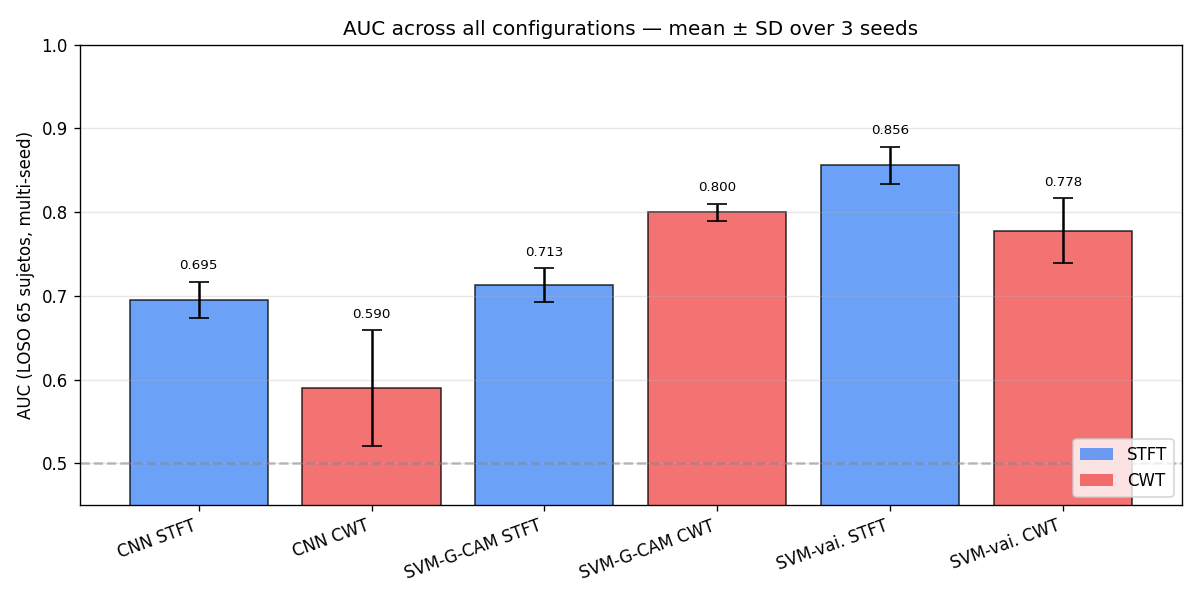
\includegraphics[width=\linewidth]{figures_informe_final/auc_master_summary.png}\\[2pt]
{\scriptsize AUC media $\pm$ SD entre 3 seeds, 6 configuraciones.}
\end{column}
\begin{column}{0.44\textwidth}
\small
\begin{itemize}
    \item Mejor configuración: \textbf{SVM vainilla + STFT}
    (la \emph{fiel al paper}):
    \[
    \text{AUC} = \mathbf{0.856 \pm 0.022}
    \]
    \item En el rango del paper original
    ($\text{Acc}\ 0.71 \pm 0.02$), sobre \textbf{datos públicos
    independientes}.
\end{itemize}

\vfill
\begin{block}{La pregunta que sigue}
\small STFT tiene \textbf{mayor AUC media} que CWT
($0.856$ vs $0.778$). \\
\textit{Pero ¿esa diferencia es real, o es ruido entre semillas?}
\end{block}
\end{column}
\end{columns}

\vfill
\centering\small
\textbf{Replicación funcional: exitosa.} Antes de afirmar que una
transformada gana, hay que probarlo bien.

\end{frame}

% ============================================================
% SLIDE 5: El giro (rigor)
% ============================================================
\begin{frame}{El giro: el rigor me obligó a frenar --- dos veces}

\begin{columns}[T]
\begin{column}{0.50\textwidth}
\textbf{Freno 1 --- La estadística.}
\small La inferencia correcta es DeLong AUC \textbf{por seed}
(preservando la varianza entre inicializaciones) y combinando con
Stouffer/Fisher, con corrección BH-FDR:

\begin{table}
\centering
\scriptsize
\begin{tabular}{l c c}
\toprule
Comparación (vainilla) & $p$ (Stouffer) & BH-FDR $q$ \\
\midrule
SVM STFT vs CWT      & $0.061$ & $0.102$ \\
SVM Grad-CAM STFT vs CWT & $0.068$ & $0.102$ \\
CNN STFT vs CWT      & $0.266$ & $0.266$ \\
\bottomrule
\end{tabular}
\end{table}
\centering\footnotesize\textbf{Ninguna comparación sobrevive
($q \geq 0.10$).}
\end{column}
\begin{column}{0.47\textwidth}
\textbf{Freno 2 --- El DSP.}
\small Las dos imágenes son $45\times45$, pero su \emph{eje de
modulación} no mide lo mismo:

\begin{table}
\centering
\scriptsize
\begin{tabular}{l c c}
\toprule
 & STFT & CWT \\
\midrule
Nyquist mod. & $\mathbf{1.56}$ Hz & $100$ Hz \\
Rango real   & $[0, 1.56]$ & $[0, 22.5]$ Hz \\
\bottomrule
\end{tabular}
\end{table}

\vfill
\begin{alertblock}{Conclusión honesta}
\small La comparación STFT vs CWT \textbf{no es concluyente} --- y
además está \textbf{confundida por DSP}. No es una comparación justa
entre transformadas.
\end{alertblock}
\end{column}
\end{columns}

\end{frame}

% ============================================================
% SLIDE 6: Lo que de verdad encontré
% ============================================================
\begin{frame}{Lo que de verdad encontré}

\begin{columns}[T]
\begin{column}{0.46\textwidth}
\centering
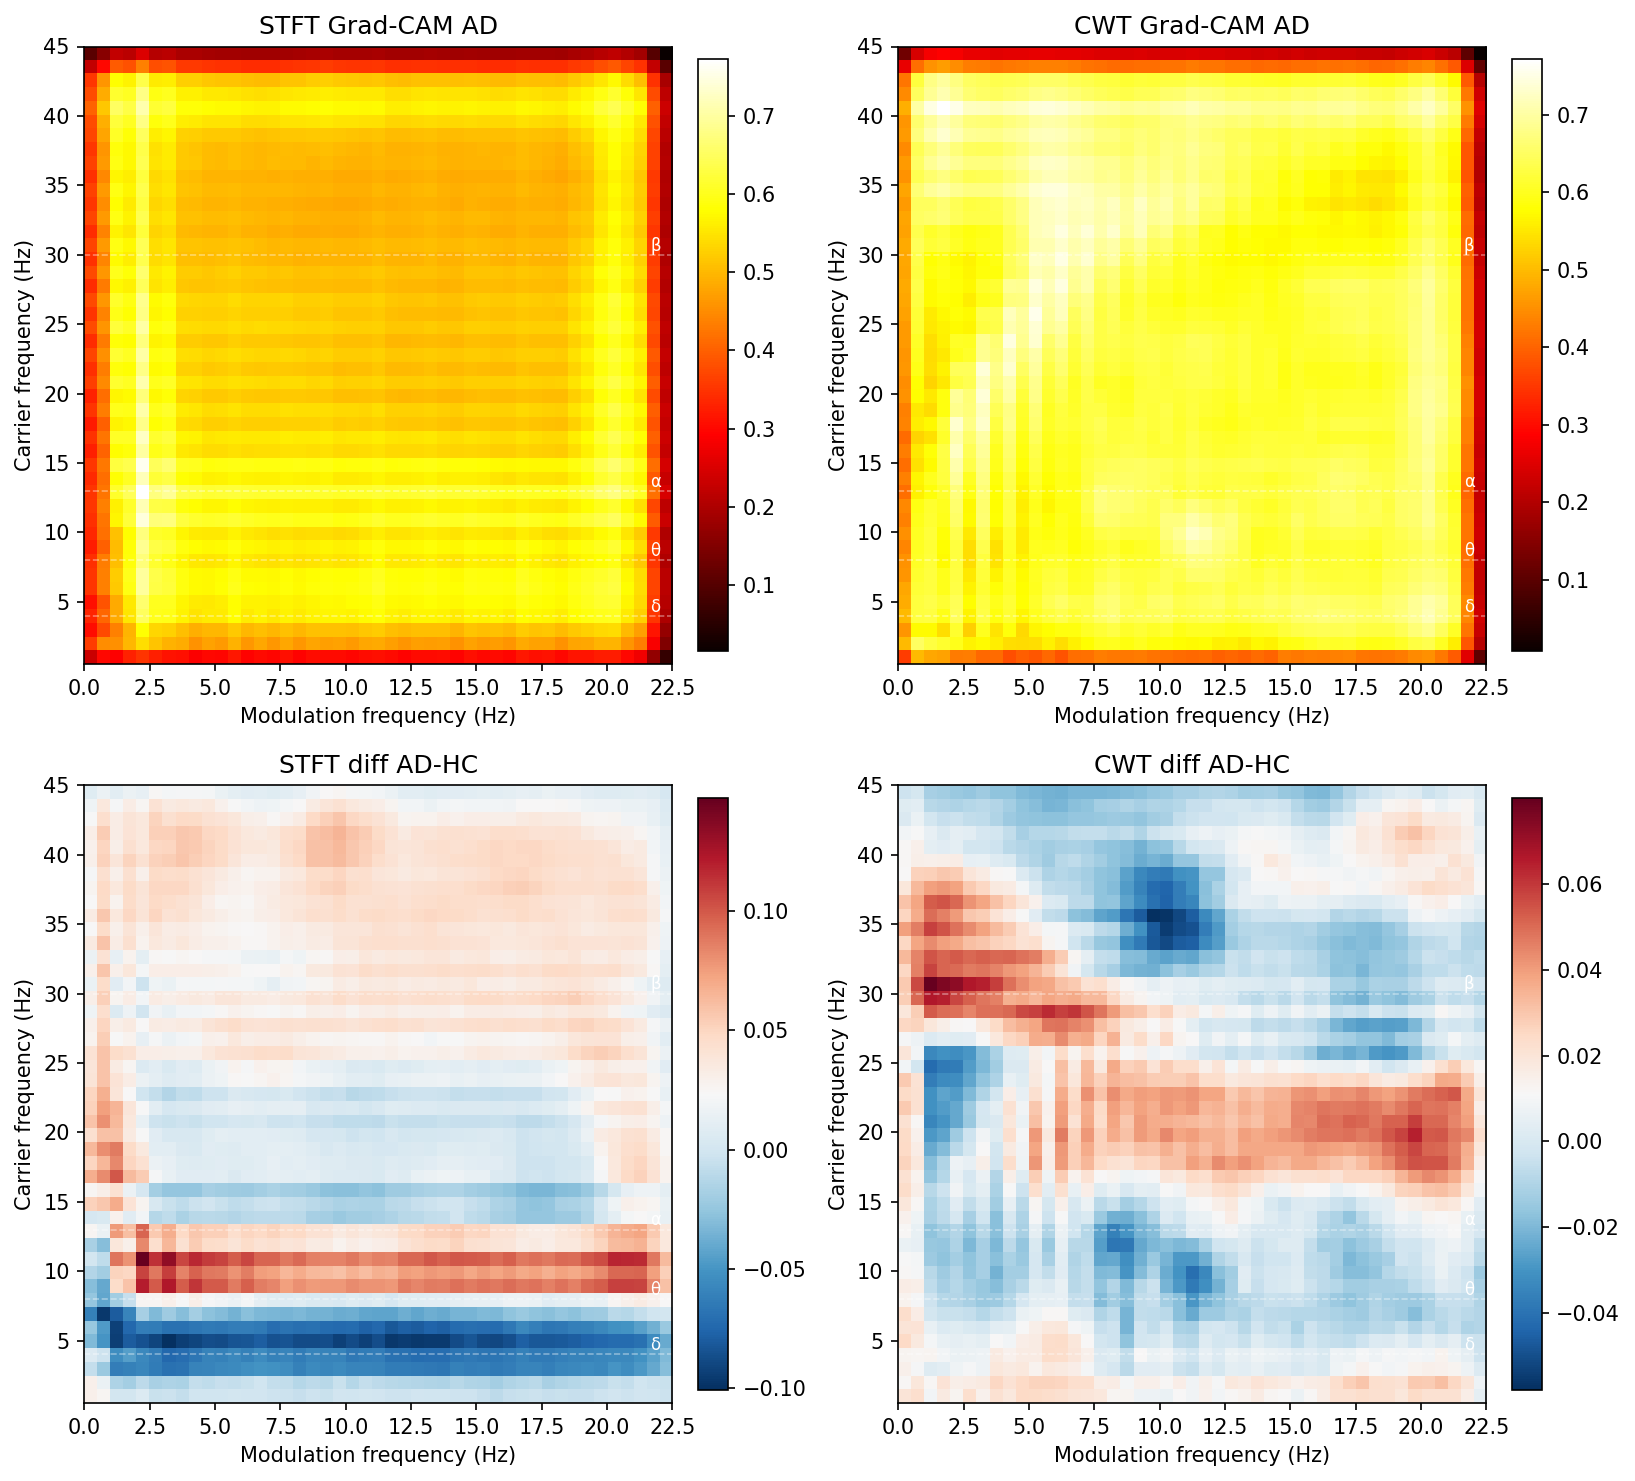
\includegraphics[width=\linewidth]{figures_informe_final/saliency_compare.png}\\[2pt]
{\scriptsize Saliency (vainilla): STFT y CWT miran regiones distintas.}
\end{column}
\begin{column}{0.50\textwidth}
\begin{enumerate}
    \item \textbf{El método de saliency cambia el ranking}: con
    Grad-CAM, CWT parece ganar; con vainilla, STFT. \\
    Los mapas son \textbf{estadísticamente ortogonales}
    ($r \approx -0.09$) $\Rightarrow$ \emph{posible complementariedad}
    (idea de ensemble a futuro).

    \vfill
    \item \textbf{El modelo redescubre biología conocida}: STFT
    vainilla concentra $\sim$89\% de su atención en bandas
    $\boldsymbol{\alpha + \theta}$ y canales
    \textbf{occipito-temporales} (O1, O2, T5, T6) --- justo donde la
    clínica localiza el Alzheimer.
\end{enumerate}
\end{column}
\end{columns}

\vfill
\centering\small
El \emph{qué} descubre el modelo depende del pipeline completo, no solo
de la transformada. \textit{Ese fue el hallazgo más interesante.}

\end{frame}

% ============================================================
% SLIDE 7: Lo que me llevo + cierre
% ============================================================
\begin{frame}{Lo que me llevo}

\begin{columns}[T]
\begin{column}{0.60\textwidth}
\begin{enumerate}
    \item \textbf{La replicación funciona} sobre datos públicos ---
    el método de Lopes es reproducible.
    \item \textbf{La hipótesis CWT $>$ STFT no se sostiene}\ldots pero
    la contraria tampoco: el rigor manda.
    \item \textbf{Lecciones metodológicas} más valiosas que el
    resultado: reportar varianza por seed, elegir bien el estadístico,
    y comparar transformadas solo con ejes equivalentes.
\end{enumerate}

\vfill
\small\textbf{Lo primero a futuro}: unificar el eje de modulación
antes de volver a comparar STFT vs CWT.
\end{column}
\begin{column}{0.36\textwidth}
\begin{block}{Reproducibilidad}
\small
\begin{itemize}
    \item Repo público, 3 seeds fijas.
    \item Anti-leakage estricto LOSO.
    \item Informe + auditoría externa.
\end{itemize}
\end{block}
\centering
{\scriptsize\url{github.com/spalaciobe/tps-alzheimer-modspec}}
\end{column}
\end{columns}

\vfill
\centering
{\Large\bfseries Gracias} \quad ---\quad \normalsize preguntas
bienvenidas.

\end{frame}

\end{document}
